\documentclass[../thesis.tex]{subfiles}
% \graphicspath{{\subfix{../Images}}}
\graphicspath{{../Images/}}

% Documents that contain labels for references in this chapter
\myexternaldocument{Sections/Introduction}

\begin{document}
\section{Neural Networks}
% Table next to figure: https://tex.stackexchange.com/questions/6850/table-and-figure-side-by-side-with-independent-captions
\begin{figure}
% \renewcommand{\figurename}{Fig.}
\renewcommand{\thefigure}{\alph{figure}}
    \begin{floatrow}
        \ffigbox[0.4\textwidth]{
\includegraphics[width=.5\linewidth]{Images/00000.png}}{
            \caption{Image from the MNIST dataset}
            \label{fig:MNIST_fig}
        }
        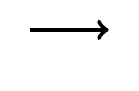
\begin{tikzpicture}[baseline=-\baselineskip]
            \draw[ultra thick,->] (0,0) -- ++ (1,0);
        \end{tikzpicture}
        \ffigbox[0.4\textwidth]{\subfile{../Tables/MNIST28x28}}{
            \caption{Image converted to $28 \times 28$ matrix}
            \label{fig:MNIST_28_28matrix}
        }
    \end{floatrow}
    \begin{floatrow}
        \qquad\qquad\qquad\qquad\qquad\qquad\qquad\qquad\qquad\qquad\qquad
        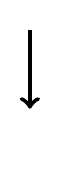
\begin{tikzpicture}[baseline=-\baselineskip]
            \draw[ultra thick,<-] (0,0) -- ++ (0,1);
        \end{tikzpicture}
    \end{floatrow}
    \begin{floatrow}
        \ffigbox[0.4\textwidth]{\subfile{../Tables/MNISToutput}}{
            \caption{Output of the NN of length 10 with on each entry the  probability that the image represents that digit.}
            \label{fig:MNIST_28_28output}
        }
        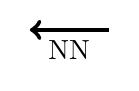
\begin{tikzpicture}[baseline=-\baselineskip]
            \draw[ultra thick,<-] (0,0) -- ++ (1,0);
            \draw (0.2,-0.1) node [anchor=north west][inner sep=0.75pt]   [align=left] {NN};
        \end{tikzpicture}
        \ffigbox[0.4\textwidth]{\subfile{../Tables/MNIST28dot28}}{
            \caption{Transposed input of NN: image converted to $28 \cdot 28$ matrix}
            \label{fig:MNIST_28_dot_28}
        }
    \end{floatrow}
\end{figure}
The goal of ML is to imitate the human brain to let a computer 'learn' a task without programming task-specific rules. One way to achieve ML is through a NN. A NN is a network that is given an input and evaluates this input to calculate an output without general knowledge of the input. The input of a NN is typically a vector containing numerical data, and the output is a vector that gives insight on the input data. The input vector can represent different types of data. How the output vector should be interpreted is dependent of the task of the NN. For classification tasks, the output vector typically contains the likelihood of the input being a class. For example, in the MNIST benchmark \parencite{lecun1998} the dataset contains pictures of the handwritten digits $0, 1, ... 9$ (figure \ref{fig:MNIST_fig}) in the form of a $28 \times 28$ matrix (figure \ref{fig:MNIST_28_28matrix}). The input vector for the NN is in this case the image matrix converted to a vector with length $28 \cdot 28$ (figure \ref{fig:MNIST_28_dot_28}). The output vector is of length 10: for each digit the likelihood of the picture being that digit (figure \ref{fig:MNIST_28_28output}). The classification of the digit on the picture is done by choosing the digit that correlates to the highest likelihood in the output vector.

A NN consists of one or several neurons. A neuron typically consist of a list of weights $w_0, ..., w_n \in \mathbb{R}$ and a bias $b \in \mathbb{R}$ and a non-linear activation function $f: \mathbb{R} \to \mathbb{R}$. The neuron receives the input vector $x_0, ..., x_n \in \mathbb{R}$ and computes $y = x_0w_0, ... x_nw_n + b$. The output of the neuron is the activation function applied on $y$. The activation function f often is the sigmoid function $\sigma (y) = 1/(1+e^{-y})$, the $\tanh$ function or the ReLU function $\textrm{ReLU}(y) = \textrm{max}(0,y)$. Another representation of a neuron is the dot product between the input and the weight vector with $b$ being one of the elements in the weight vector and constant value $1$ being the corresponding element in the input vector. 

% NN is evaluated on input and gives an output. Typically vectors. NN has input (numerical data) vector and an output vector that typically gives insights on input vector. Input can represent different types of data: MNIST [source] input is 28x28 input of grayscale pictures of handwritten digits 0..9. An MxN grayscale input can be represented as a MdotN matrix and rgb as 3dotMdotN matrix. 
% How the output can b interpreted is dependend of the task of the NN. When used for classification the output often is displayed as the change of the input being classified of the different possibilities. When difference between cat and dog, the output is of length 2 and the input is classified as the class from the highest number in the output vector. 
% Deeplearning often used for classification - achieved by the possibility what digit has the highest possibility
% A NN is often used to "learn" to perform tasks like classification, generally without programming task-specific rules, meaning that you could use the same neural network and train it on another dataset. For classification of cats: they do it without general knowledge of cats, for example: fur tails and whisker.

% NN consist of neuron: containing set of weights w0, wn set of real numbers and bias b set of real numbes. It gets as input list of number x0,...,xn set of real numbers and calculates y = x0w0, ... xnwn + b and then applies non linear activation function f: r -> r to compute output z = f(y). Another representation is dot product between inptu and weight vector with b being an element of the weight vector and constant signal 1 being corresponding element in the input vector. Activation function often signmoid or the ReLU function. 

NNs have sequences of layers containing one or more neurons. The first layer contains the input of the NN and the last layer is the output. Layers in between are one or more 'hidden layers'. The neurons in a layer are connected to neurons on other layers: the output of a neuron can be connected to the input of other neurons in other layers. The network created is a directed weighted graph. Each link in the graph has a weight, it determines the strength of a neurons connection to another. The neurons can be connected in different ways. In a fully connected NN all nodes in a layer are connected to all the neurons in the next layers. When the output of the neurons in layer $i$ are connected to layer $i+1$ the network is called a feed-forward NN. Networks that also allow connections to previous layers are called recurrent networks. Some of the typically used layers are fully-connected (FC) layers, convolutional (Conv) layers\footnote{Convolutional layers play an important role in convolutional neural networks (CNNs) that are widely used in networks used for image processing tasks}, activation layers and pooling layers. FC and Conv layers apply a linear function on their input and hence are called linear layers. Most other layers are non-linear. 

% NNs have seqeuence of layers of neurons. First layer contains input of NN output of last layer of NN is result of NN. Layers inbetween are hidden layers composed of neurons. The hidden layer can contain zero or more layers. the neurons in this layers are connected to neurons on other layers: the output of some neurons are the input of other neurons.  The network created is a directed weighted graph. each link in the network has a weight, it determines the strength of ones node to another. THe neurons in the network can be connected in different ways. In a fully connected Neural network all nodes in a layer are connected to all the neurons in the next layers. In a feedforward neural network The output of layer i is fed into layer i+1. Networks that allow connections to previous layers are calleed recurrent networks. 

% Layers:
% Fully-connected (FC) layer: Contains a matrix of weights. Computes the output vector by multiplying the input vector with the weight matrix.
% – Convolutional (Conv) layer: Contains a set of weight matrices called feature maps that are smaller
% than the input. Computes output numbers by sliding a window of the size of the feature map
% over the input, and computing the dot product of the feature map with the part of the input in
% the sliding window. Conv layers play an important role in convolutional neural networks (CNNs),
% which are widely used in image processing tasks.
% – Activation layer: Applies the same R → R activation function to each element of the input to
% compute the elements of the output. Depending on the function, there can be ReLU activation
% layers, tanh activation layers, etc.
% – Pooling layer: Computes output numbers by sliding a window of size k over the input, and applying
% an R
% k → R pooling function. The most common pooling function is the max function, resulting in
% a Max-Pool layer.

% FC and conv layers are linear layers because they apply linear function on their input to calculate output. Most of the other layers are non-linear. 

To create a NN one must first determine its architecture: what number and types of layers should it contain, in what order should the layers be and what are the sizes of the layers. Some layers change the size of their input and can thus create a degree of freedom. Next, the network has to be trained. During the training the parameters of the layers (for example the weights in the FC layer) are iteratively tuned, typically by calculating the difference between the calculated output (that often is a prediction) and the target output. This is done by applying data on the NN where the output is already known (e.g. manually labeled). After training the network it is used for the inference phase where new input is applied to the NN. The accuracy of the NN is tested on new data where the output is also known, typically a dedicated subset of the training data. The accuracy is then defined as the ratio between the correctly labeled output (in terms of expected output of the NN) and mislabeled output.

% A NN is created first by determining the architecture: the number and types of layers, their order, and sizes. Some layers (FC, conv, and pooling layers change the size of their input thus creating degree of freedom)

% Next, the NN has to be trained. During training the parameters of the layers are being iteratively tuned. Typically by calculating the difference between the calculated output (often a prediction) and a target output.  constantly changed to change the output and get it as matching as possible with the expected output. This is done by applying data on the NN where the output is already known (e.g. manually labeled).

% After training the NN is used for inference stage where the NN will be applied to new input. The NN is tested on a part of the training dataset that will be kept seperated where the output is known from. Using a dedicated validation of the training dataset. Accuracy is the verhouding tussen the input where the output is the expected output. A subset of the training data is kept aside for testing the accuracy of the NN

\section{Secure Neural Networks Inference}
The hidden layers contain all the information of the NN. After the tedious process of training the model one often wants to keep the parameters of the hidden layer secret. Besides, the model can reveal information about the training data \parencite{qayyum2020} which in turn can also contain privacy sensitive information. This and the aforementioned reasons result in the SNNI problem in the case of MLaaS. Solving this problem is quite challenging. Some approaches have been suggested with cryptographic techniques like homomorphic encryption \parencite{rivest1978} and secure multi party encryption \parencite{yao1982, yao1986}. Other hardware based approaches have also been suggested \parencite{deepsecure}. All approaches achieve different trade-offs in terms of accuracy, security, efficiency and applicability. 

Several authors have tried to make an overview on privacy preserving ML. Tanuwidjaja et. al. (\citeyear{tanuwidjaja2020}) have done a comprehensive survey on MLaaS in general and have given a chronological overview of the works. Mann et. al. (\citeyear{mann22}) have summarized the work on the inference part of ML. The approaches that I will test have been chosen from this paper, since it is the most recent overview on the field of SNNI. It also provides substantial information about the approaches, and I could therefore make an informed choice on the approach to test.  

\section{Cheetah}
Cheetah is a hybrid model, which means it uses different primitives for the linear functions and for the non-linear functions. Here I will give a short overview of the techniques used for Cheetah and the design choices of the authors. For a more in-depth explanation, I refer the reader to the original paper \parencite{cheetah}. \paragraph{}

Most cryptographic protocols use additive secret sharing techniques to switch back-and-forth between different types of cryptographic protocols. The first question following is what domain should be used for the additive sharing, the ring $\mathbb{Z}_{2^l}$ or prime field $\mathbb{Z}_{p}$. Oblivious transfer (OT) protocols, used for the non-linear part of Cheetah, perform better on the ring $\mathbb{Z}_{2^l}$ than on prime field $\mathbb{Z}_{p}$ and modulo reduction in $\mathbb{Z}_{2^l}$ is almost free. However, most homomorphic encryption (HE) based protocols used in practice force to export the additive secret to the less efficient $\mathbb{Z}_{p}$ because of the Single-Instruction-Multiple-Data (SIMD) techniques they heavily utilize. One can use several techniques to accept secret shares from $\mathbb{Z}_{2^l}$ at the cost of increasing overhead and ruining the gains of the non-linear part. The authors tried to get both: amortized homomorphic operations while keeping the efficient non-linear protocols without extra overhead \parencite[p 810]{cheetah}.

It is inevitable for the prior HE-based and SIMD-tailored protocols to rotate operands, which is an expensive operation, many times due to the spatial property. The authors present three pairs of encoding functions to evaluate the linear layers (convolution-, batch normalization- and fully connection layers) via polynomial arithmetic circuits. These functions map the input of a NN to (a) polynomial(s). By carefully choosing the proper coefficients of the output polynomial(s) they eliminate the need for expensive rotations, which makes it able to accept secret shares from $\mathbb{Z}_{2^l}$. This also helped reduce the cost of other homomorphic operations. 

With the advent of silent OT, based on vector oblivious linear evaluation (VOLE), many communication efficient OT extensions are proposed by other authors. But these extensions do not always achieve best performance. Take for example the Millionaire protocol for integer comparison: only upgrading the OT extensions with VOLE does not always achieve speedup. Improvements to this protocol are made in Cheetah. Further improvements are made to the expensive truncation protocol (which contributes to more than 50\% of the communication overhead in CrypTFlow2).  

% with advent of silent ot extension many communication ot extensions are proposed. But it does not always achieve best performance, for example with the millionaire protocol.

% Improvements to trunctation protocol which is rquired after each multiplication so that the fixed point values will not overflow. First by not touching one of the two probability errors because it barely harms the inference results. Secondly because sometimes the Most significant bit is somtimes already known.

% Polynomial multiplication can be viewed as a batch of inner products if we arrange the coeficients properly. They introduce natural mappings $\pi^i_\mathcal \pi^w_\mathcal$ to properly place the values in the input and weight to polynomial coefficients for each of the $\mathcal \in {CONV, BN, FC}$ [[[[[[[[[[dit nog ff checken of het wel e symbool is ]]]]]]]]. 

% \subsection{lattice based homomorphic encryption}
% HE that is based on learning with errors (LWE) and its ring variant (ring-LWE). 

% \color{red} \textbf{Only draft text or notes from me from this point}
% \color{black}\newline
% Is hybrid model i.e. it uses different primitives for linear function and other for non-linear functions.
% cheetah achieves performmance by codesing of dnn, lattice-based homomorphic encryption, bolivious transfer and secret-sharing

% Here i will give a short overview on the techniques used in cheetah. For a more in depth explanation and design choices i refer the reader to the original paper. 

% The first question is waht domain should be used for additive sharing to switch back-and-forth between different types of cryptographic primitives. OT-based protocols based on the ring $Z_{2^l}$ perform better than protocols based on $Z_p$. State-of-the-art HE-based protocols force to export to $Z_p$ because these protocols heavily utilize the homomorphic Single-Instruction-Multiple-Data (SIMD) technique to amortize the cost. One can use techniques to accept $Z_{2^l}$ at the cost of increasing overhead and ruining the gains of the non-linear part.  
% Authors tried to get the best of two worlds: amortized homomorphic operations while keeping the efficient non-linear protocols without extra overhead

% They did this by improving CrypTFlow2 using smart techniques. 

% \subsection{Fast and SIMD free linear protocols}
% Due to spatial property of the convolution and matrix-vector multiplicaation it is inevitable for the prior he-based and simd protocols to rotate the operands many times. Because it is expensive(?). THus the authors of Cheetah designed their linear layers (conv, bn, fc) via polynomial arithmetic circuits which maps the values of the input to the proper coefficients of the output polynomial(s). 
% \begin{quote}
%     \emph{"By careful design of the coefficient mappings, we not only eliminate the expensive rotations but are also are able to accept secret shares from $Z_{2^l}$ for free"} \parencite[p. 810]{cheetah}
% \end{quote}

% This also helps to reduce the cost of other homomorphic operations (e.g. encryption and decryption). It can also use large lattice dimension and also smaller. 

% \subsection{Leaner protocols for the non linear functions}
% with advent of silent ot extension many communication ot extensions are proposed. But it does not always achieve best performance, for example with the millionaire protocol.

% Improvements to trunctation protocol which is rquired after each multiplication so that the fixed point values will not overflow. First by not touching one of the two probability errors because it barely harms the inference results. Secondly because sometimes the Most significant bit is somtimes already known.

% Polynomial multiplication can be viewed as a batch of inner products if we arrange the coeficients properly. They introduce natural mappings $\pi^i_\mathcal \pi^w_\mathcal$ to properly place the values in the input and weight to polynomial coefficients for each of the $\mathcal \in {CONV, BN, FC}$ [[[[[[[[[[dit nog ff checken of het wel e symbool is ]]]]]]]]. 

% \subsection{lattice based homomorphic encryption}
% HE that is based on learning with errors (LWE) and its ring variant (ring-LWE). 

\section{CrypTFlow2}
One of the problems that the authors of CrypTFlow2 encountered in prior works was that the existing secure 2-party computation (2PC) protocols used ReLU activation\footnote{Relu(\textit{x}) is defined here as max(\textit{x},0)} layers, which are expensive to compute securely. Efficient approaches to evaluate ReLu layers require a sacrifice in terms of security, which is not desirable. A second problem was that prior works fail to provide a faithful implementation of secure fixed point-arithmetic, which is necessary to preserve inference accuracy. When fixed-point arithmetic is not correct errors are propagated through the networks, resulting in an output that is arbitrary far from  the desired output. \paragraph{}

Their first contribution is a improved protocol for the millionaires problem\footnote{The problem where two parties, $P_0$ and $P_1$ each hold an integer, $x$ and $y$ respectively and want to securely compute $x<y$}. The first improvement is modifying the tree so recursion is done log($l/m$) times to obtain strings of size $m$ for bit length $l$. Then a 1-out-of2$^m$ OT is used at the leaves, using a lookup-table based approach. Apart from this they also carefully changed the sender's and receiver's message to combine 1-out-of-2$^m$ instances and reduce communication.  

With this improvement to the millionaires problem, the authors built new protocols for computing DReLU\footnote{The derivative of the ReLU function} for both the ring $Z_{2^l}$ and general rings $Z_n$. DReLU serves as a building block more efficient division over both domains as for the non-linear activation functions like ReLU and Maxpool. Supporting both $Z_{2^l}$ and $Z_n$ domains allows the authors to evaluate the linear layers using HE and OT. 

The next contribution, regarding faithful fixed-point arithmetic, is that the authors provide new protocols for division by power-of2 as well as division by arbitrary integers. These protocols provide a correct solution to fixed-point arithmetic. One other approach is via garbled circuits, but these protocols are $\approx 54$x less efficient than the new protocols in terms of communication. 

prior works have discussed the OT vs HE conundrum. Initial works have used OT-based protocols because they require less computation than HE-based protocols, but the state-of-the art protocols, with better inference latency, use HE-based protocols because they require less communication. To resolve the empirical question of what protocols are better, the authors build CrypTFlow2, containing two classes of protocols $SCI_{HE}$ (for the HE-based protocols) and $SCI_{OT}$. (for the OT-based protocols). The observations were that in WAN setting, where communication is a bottleneck, HE-based protocols were faster, and in LAN setting OT and HE are incomparable. For this research we will hence use $SCI_{HE}$. I will use $SCI_{HE}$ and CrypTFlow2 interchangeably from this moment.
\end{document}